\documentclass[11pt]{article}
\usepackage [french]{babel}
\usepackage [T1]{fontenc}

\usepackage[linesnumbered, ruled, french, onelanguage]{algorithm2e}
\usepackage{amssymb}
\usepackage{amsmath}
\usepackage{adjustbox}%Permet de centrer les figures dans la largeur de la page même si les figures sont plus larges que \textwidth
\usepackage{xcolor}%/definecolor et /color
\usepackage{graphicx}
\usepackage{geometry}%Pour changer la largeur des marges du document notamment
\usepackage{placeins}%pour utiliser FloatBarrier afin que les figure respectent bien leur position dans le code
\usepackage{gensymb}%pour pouvoir écrire le signe °
\usepackage{hyperref}%pour les liens dans la bibliographie
\usepackage{stmaryrd}%pour les crochets à double barres d'intervalles de nombre entiers
\usepackage{listings}
\usepackage{slashbox}%Case séparée en deux tout en haut à gauche des tableaux à double entrées

%%%%%%%%%%%%%% Couleurs de: https://texblog.org/2011/06/11/latex-syntax-highlighting-examples/ %%%%%%%%%%%%%%
\definecolor{javared}{rgb}{0.6,0,0} % for strings
\definecolor{javagreen}{rgb}{0.25,0.5,0.35} % comments
\definecolor{javapurple}{rgb}{0.5,0,0.35} % keywords
\definecolor{javadocblue}{rgb}{0.25,0.35,0.75} % javadoc
 
\lstset
{
language=Java,
keywordstyle=\color{javapurple}\bfseries,
stringstyle=\color{javared},
commentstyle=\color{javagreen},
morecomment=[s][\color{javadocblue}]{/**}{*/},
numbers=left,
numberstyle=\tiny\color{black},
stepnumber=1,
numbersep=10pt,
tabsize=4,
showspaces=false,
showstringspaces=false}
%%%%%%%%%%%%%% Couleurs de: https://texblog.org/2011/06/11/latex-syntax-highlighting-examples/ %%%%%%%%%%%%%%





\author{}
\title{Ray-Tracer}
\date{}
\geometry{hmargin=3cm, vmargin=2cm}

\begin{document}
\tableofcontents
\newpage

\maketitle

\section{Détail des parties techniques}
\subsection{Le Ray Tracer}
\subsubsection{L'algorithme de base}
Dans notre vie quotidienne, nous voyons ce qui nous entoure grâce aux photons émis par les différentes sources de lumière présentent autour de nous (le soleil ou nos lumières artificielles notamment). Chaque photon émit par ces sources vient alors frapper un des objets qui fait notre environnement. Si l'on imagine par exemple une tasse en face de nous, avec une lampe au plafond, un photon partant de cette dernière viendra rebondir sur la tasse pour ensuite, éventuellement, être redirigé en direction de nos yeux. Si le photon arrive en effet jusqu'à nos yeux, c'est alors qu'on verra se dessiner la tasse devant nous. La tasse est éclairée et nous la voyons. Bien sûr, ce phénomène est, à l'échelle de l'humain, instantané et c'est pour cela que nous ne voyons pas notre environnement apparaître progressivement devant nous chaque fois que nous allumons notre lumière. \\
L'objectif d'un algorithme de ray-tracing est de calculer le rendu d'une scène 3D d'une façon similaire à celle qui nous permet de voir tous les jours. En effet, nous pouvons faire un parallèle entre notre algorithme de ray-tracing et la vie à laquelle nous sommes habitués grâce à 3 composants principaux:
\begin{itemize}
	\item{Une scène composée d'objets (sphères, plans, triangles, ...) que l'on peut comparer à notre environnement}
	\item{Une (ou plusieures) sources de lumière jouant le même rôle que nos sources de lumière habituelles}
	\item{Une caméra représentant nos yeux}
\end{itemize}
Une différence notable avec ce qui nous permet de voir dans la vie de tous les jours est que nos rayons (ou photons) partiront de la caméra (nos yeux) plutôt que de la source de lumière. Nous faisons en quelque sorte le chemin inverse. En lançant un rayon au travers de chaque pixel de l'image que nous voulons calculer, nous pourrons ensuite vérifier si le rayon a rencontré un objet de la scène. Dans ce cas, le pixel pourra alors être coloré de la couleur de l'objet, le rendant ainsi visible.

\begin {algorithm}[H]
	\DontPrintSemicolon
	\KwIn{\textit{height} la hauteur de l'image à rendre,\\\textit{width} la largeur de l'image,\\\textit{scene} la scène 3D à rendre}
	\KwOut{P un ensemble de pixels $p_{i, j}$ $\{p_{0, 0}, p_{0, 1}, \ldots, p_{height-1, width-1}\}$, $i$, $j \in \mathbb{N}$, $0 \leqslant i \leqslant height-1$, $0 \leqslant j \leqslant width-1$\\\hfill\\}

	$O \gets Origine\ de\ la\ camera$\\
	\For {$y \gets 0$ \textbf{to} $height$} 
	{
		\For {$x \gets 0$ \textbf{to} $width$} 
		{
			$C_{y, x} \gets convPxCoToWorldCoords(x, y)$\\
			$\overrightarrow{ray} \gets \overrightarrow{OC_{y,x}}$\\
			\hfill\\
			$p_{y, x} \gets lancerRayon(\overrightarrow{ray}, scene)$
		}
	}

	\caption{Pseudo-code du lancer des rayons - rayTrace}
	\label{lancerRayons}
\end {algorithm}

\subsubsection{Conversion camera-scène}
\label{conversionCamera}

Comme le montre l'algorithme \ref{lancerRayons}, parcourir chaque pixel ne suffit pas. Si l'on souhaite lancer un rayon depuis la caméra à travers le pixel que l'on cherche à colorer, il nous faut les coordoonnées de ce pixel exprimées dans l'espace 3D de la scène.\\
Prenons l'exemple du rendu d'une image dans une résolution 800x600 pixels. Si l'on veut calculer la couleur du pixel de coordonnées $P = (430, 256)$ sur l'image, construire un rayon d'origine $O$ la caméra et de direction le vecteur $\overrightarrow{d} = \overrightarrow{OP}$, n'est pas une solution viable. En effet, le point $P$ n'est pas exprimé dans les coordonnées de notre scène où se trouvent nos objets. Il est exprimé dans les coordonnées de l'image. Nous avons donc besoin de faire correspondre les coordoonnées d'un pixel de l'image à ses coordoonnées dans le monde:

\begin {algorithm}[H]
	\DontPrintSemicolon
	\KwIn{$x, y \in \mathbb{N}$, les coordonnées du pixel sur l'image,\\
		$width, height$\ la\ largeur\ et\ la\ hauteur\ de\ l'image\ à\ rendre,\\
		$F \in\ ]0; 180[$\ le\ champ\ de\ vision\ de\ la\ caméra\ (FOV)\ en\ degré}
	\KwOut{$P_{world}(x_{world}, y_{world}, -1)$\\le\ point\ dont\ les\ coordonnées\ représentent\ celles\ du\ pixel\ exprimées\ dans\ l'espace\ de\ la\ scène.\\\hfill\\}

	$aspectRatio \gets width/height$\\
	$F_{rad/2} \gets \frac{F}{2}*\frac{\pi}{180}$\\
	$demiPlaneHeight \gets tan(F_{rad/2})$\\
	\hfill\\
	$x_{world} \gets x$\\
	$y_{world} \gets y$\\
	\hfill\\
	$x_{world} \gets (x_{world} +0.5) / width$		{\tcp*[f]{Etape 1}}\\
	$x_{world} \gets x_{world} * 2 -1$ 			{\tcp*[f]{Etape 2}}\\
	$x_{world} \gets x_{world} * demiPlaneHeight$ 	{\tcp*[f]{Etape 3}}\\
	$x_{world} \gets x_{world} * aspectRatio$		{\tcp*[f]{Etape 4}}\\

	\hfill\\
	$y_{world} \gets (y_{world} +0.5) / height$ 		{\tcp*[f]{Etape 1}}\\
	$y_{world} \gets 1 - y_{world} * 2$ 			{\tcp*[f]{Etape 2}}\\
	$y_{world} \gets y_{world} * demiPlaneHeight$ 	{\tcp*[f]{Etape 3}}\\

	\hfill\\
	\Return{$(x_{world}, y_{world}, -1)$}

	\caption{Conversion des coordonnées d'un pixel de l'image aux coordonnées de la scène - conversionPixelScene}
	\label{conversionPixel}
\end{algorithm}

Il est important de remarquer que notre caméra se trouve initialement aux coordonnées $O = (0, 0, 0)$ et que sa direction de regard est $\overrightarrow{d_{cam}} = (0, 0, -1)$. Par convention, la grille de pixel virtuelle (le plan de la caméra) à travers laquelle nous faisons passer nos rayons se trouve à 1 unité de distance de la caméra, dans sa direction de regard. Ainsi, la coordonnée z des pixels sera toujours -1.\\
\begin{figure}[h!]
	\adjustbox{center}{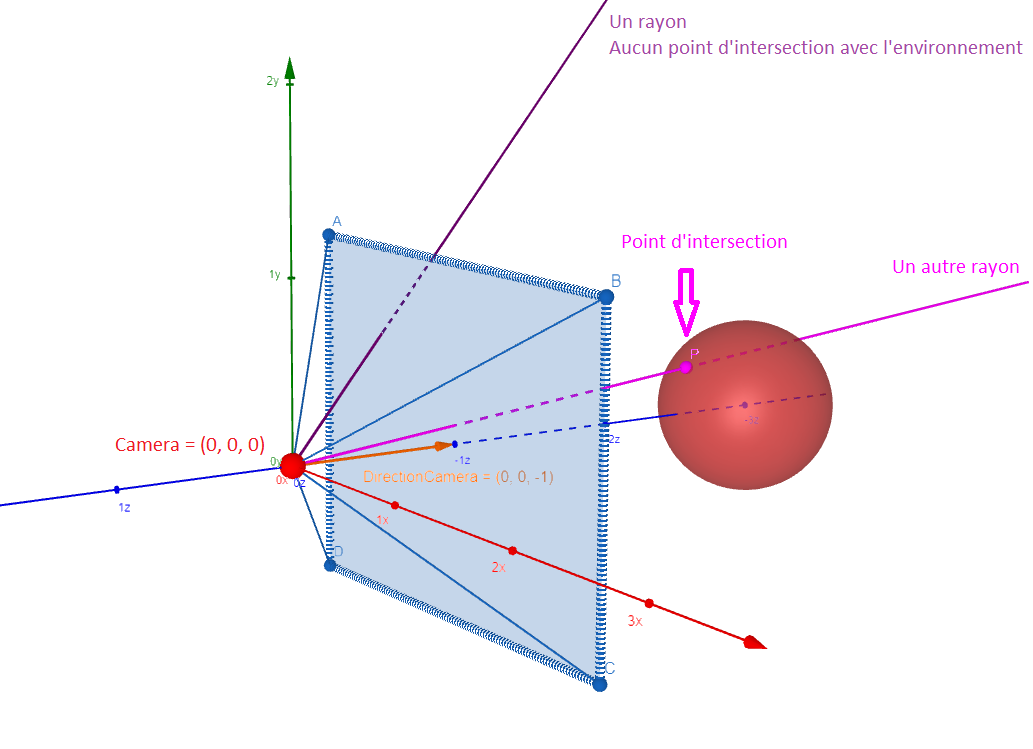
\includegraphics[width=1.1\textwidth]{img/rt/repCam2Rayonsv2.png}}

	\caption{Représentation de la caméra, de son plan, de sa direction ainsi que d'une sphère représentant l'environnement. Deux rayons sont également tracés.}
	\label{repreCamRayon}
\end{figure}
\FloatBarrier

En reprenant l'exemple de notre image de rendu en 800x600 pixels et en suivant les étapes de l'algorithme \label{conversionPixel}:\\
$P(x, y, z), x \in [0; 799], y \in [0; 599], z = -1$ :
\begin{enumerate}
	\item{\textbf{Etape 1} : On ajoute 0.5 à la valeur du pixel que l'on veut rendre. Les pixels étant des carrés de 1x1 unité sur l'image, ajouter 0.5 fera donc passer le rayon au centre du pixel. La division par la largeur et la hauteur de l'image (pour x et y respectivement) permet de ramener les coordonnées des pixels dans l'intervalle $[0; 1]$.\\
		\hfill\\
	         	$P(x, y, z), x \in [0; 1], y \in[0; 1], z = -1$}
	\item{\textbf{Etape 2} : Le but de cette étape est de ramener les pixels dans l'intervalle $[-1; 1]$.\\
		$x*2 \Rightarrow x \in [0; 2]$
		$\\x - 1 \Rightarrow x \in [-1; 1]$\\
		Même raisonnement pour y à une inversion d'opération prêt.\\
		\hfill\\
	          	$P(x, y, z), x \in [-1; 1], y \in[-1; 1], z = -1$}
	\item{\textbf{Etape 3} : Cette étape permet de prendre en compte le champ de vision de la caméra. Plus le champ de vision se rapproche de 180\degree, plus la caméra voit une grande partie de la scène et inversement. Le champ de vision peut alors donner une impression de "zoom". Voir plus bas la \figurename~\ref{fovCam}\\\hfill\\
		$P(x,y , z), x \in [-1; 1]*FOV, y \in [-1; 1]*FOV, z = -1$.}\\
	\item{\textbf{Etape 4} : Jusqu'alors, les coordonnées de nos pixels converties dans l'espace du monde formaient un plan de caméra carré. Comment faire si l'image que nous voulons rendre n'est pas elle-même carrée (ce qui est très fréquent) ? Il nous faut prendre en compte le format de l'image donné par $width/height$. En multipliant la coordonnée x par ce format, nous "étirons" l'image ou la rétrécissons selon sa largeur. Le plan de la caméra respecte maintenant le même format que l'image que nous voulons rendre.\\\hfill\\
		$P(x,y , z), x \in [-1; 1]*FOV*aspectRatio, y \in [-1; 1]*FOV, z = -1$.}
\end{enumerate}

\begin{figure}[h!]
	\adjustbox{center}{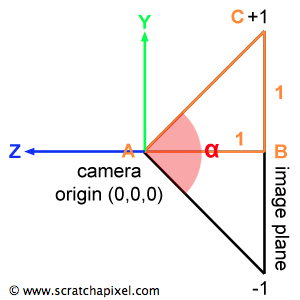
\includegraphics[width=0.5\textwidth]{img/rt/fovCamera.png}}

	\caption{En augmentant le FOV (champ de vision) de la caméra, l'angle $\alpha$ augmente. La hauteur du plan de la caméra, $BC$, est étirée. La caméra verra donc une plus grande partie de la scène. \textbf{Source: scratchapixel.com} \cite{scratchapixel}}
	\label{fovCam}
\end{figure}
\FloatBarrier

A l'issue de ces implémentations, nous obtenons alors l'image suivante (la scène est composée d'une unique sphère rouge et d'un fond gris foncé):

\begin{figure}[h!]
	\adjustbox{center}{
\includegraphics[width=0.5\textwidth]{img/rt/basicRender.png}}

	\caption{Rendu le plus simple. Une sphère sans aucun effet d'ombrage.}
	\label{basicRender}
\end{figure}
\FloatBarrier

Chaque rayon qui a été lancé et qui a intersecté la sphère a alors donné un pixel rouge. Les autres rayons, ceux qui n'ont pas intersecté la sphère, ont simplement renvoyé la couleur du fond de la scène. 

\subsubsection{L'ombrage de Phong}
\label{ombragePhong}

Comme vu précédemment, la première image (fig. \ref{basicRender}) produite par notre algorithme n'est pas tout à fait satisfaisante. Il n'y a en effet aucun effet de profondeur ou de lumière. Difficile de savoir qu'on a une sphère devant nous et non un simple disque plat. La prochaine étape est donc celle de l'ombrage de Phong. Un tel ombrage se découpe en trois composantes/parties:
\begin{enumerate}
	\item{La composante ambiante. Elle est responsable de la quantité minimale de lumière que va reçevoir un objet}
	\item{La composante diffuse. Cette composante est celle qui permet de donner à un objet son relief. Plus les rayons de la lumière arrivent perpendiculairement à la surface de l'objet, plus l'intensité lumineuse sur la surface de l'objet sera importante}
	\item{La composante spéculaire. Elle permet d'ajouter un effet "brillant" aux objets en fonction de la direction qu'empruntent les rayons réfléchis par la surface de l'objet par rapport à la caméra.}
\end{enumerate}

\hfill\\
\indent La composante ambiante permet de donner une illumination de base à l'objet. En temps normal, même si un objet n'est pas directement éclairé par la source de lumière, il est tout de même visible dans la plupart des cas. C'est parce que la lumière de la source lumineuse rebondit dans la scène et les rayons arrivent indirectement éclairer l'objet. C'est ce que l'on appelle l'illumination globale. L'illumination globale est capable de génèrer des images fortes de réalisme mais est très coûteuse en temps de calcul. La composante ambiante de l'ombrage de Phong approxime très simplement cet effet en donnat une "luminosité mininale" à toute la scène. La composante ambiante est très simple à calculer:\\

\begin{center}
	$Ambiante = I_A = S_A*I_L$
\end{center}
Avec $I_L\ \in\ [0;1]$ l'intensité de la source lumineuse,\\
$S_A\ \in\ [0; 1]$ l'intensité de la lumière ambiante dans la scène. Ce paramètre affecte donc tous les objets de la scène.

\begin{figure}[h!]
	\adjustbox{center}{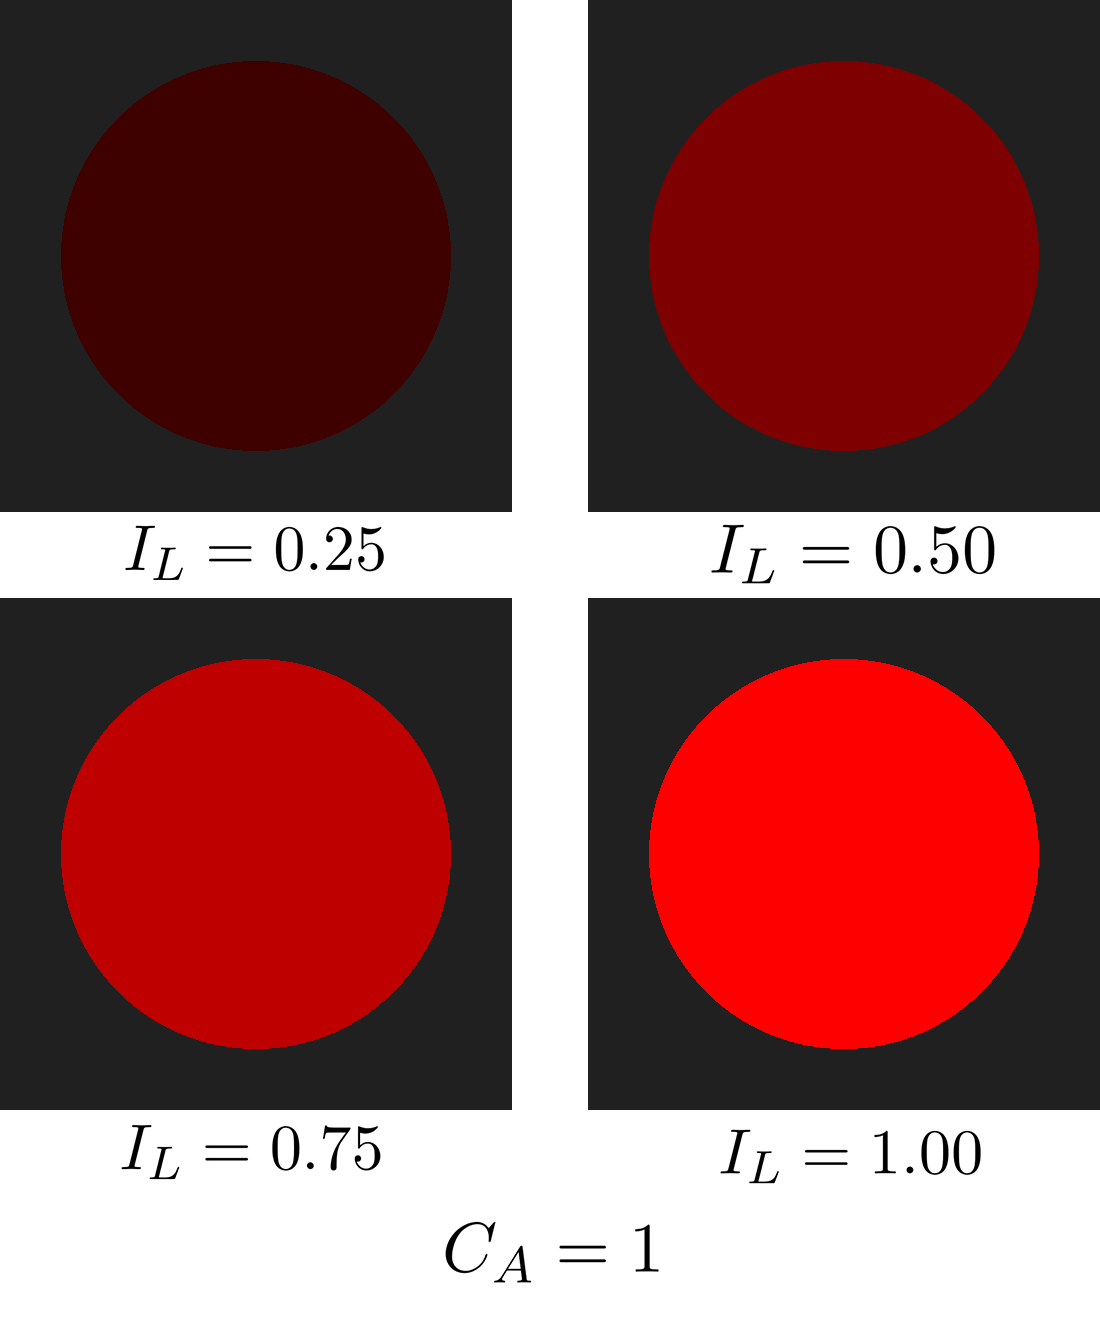
\includegraphics[width=0.5\textwidth]{img/rt/differentAmbient.png}}

	\caption{Le rendu de la même sphère pour différentes intensités lumineuse $I_L$. $C_A = 1$ utilisé pour tous les rendus.}
	\label{differentAmbient}
\end{figure}
\FloatBarrier

La composante diffuse de l'ombrage de Phong permet d'ajouter un effet que l'on peut voir comme un dégradé d'intensité lumineuse. L'intensité est à son maximum lorsque les rayons de la source lumineuse frappent perpendiculairement la surface de l'objet. Au contraire, lorsque les rayons sont parallèles à la surface de l'objet, l'intensité lumineuse de la diffusion est très faible. Elle est calculée comme suit:\\

\begin{center}
	$Diffuse = I_D = C_D*(\overrightarrow{L}\cdot\overrightarrow{N})$
\end{center}
Avec $C_D$ le coefficient d'intensité diffuse de l'objet,\\
$\overrightarrow{L}$ le vecteur en direction de la source lumineuse depuis le point d'intersection du rayon et de l'objet,\\
$\overrightarrow{N}$ la normale de la surface de l'objet au point d'intersection avec le rayon\\
et $\cdot$ dénotant le produit scalaire.\\
On sait que le produit scalaire de deux vecteurs orthogonaux est égal à 0. De plus, le produit scalaire de deux vecteurs colinéaires normalisés (de longueur 1) vaut 1. Ainisi, deux vecteurs normalisés non-colinéaires et non-orthogonaux auront un produit scalaire compris entre 0 et 1. Plus les vecteurs sont similaires, plus le produit se rapprochera de 1 et à l'inverse, "plus les vecteurs sont orthogonaux" plus il tendra vers 0.\\
Appliqué au cas de notre sphère et de notre source de lumière :\\
\begin{itemize}
	\item{Si le vecteur représentant la direction du rayon de lumière (le vecteur entre le point d'intersection sur l'objet et la source lumineuse) est colinéaire à la normale au point d'intersection de l'objet, l'intensité de la composante diffuse sera maximale car le produit scalaire des deux vecteurs vaudra alors 1.}
	\item{Si au contraire, la lumière frappe l'objet de côté, la normale et le vecteur du rayon de lumière seront alors orthogonaux (ou presque), le produit scalaire vaudra 0. L'intensité de la composante diffuse sera minimale.}
\end{itemize}


\begin{figure}[h!]
	\adjustbox{center}{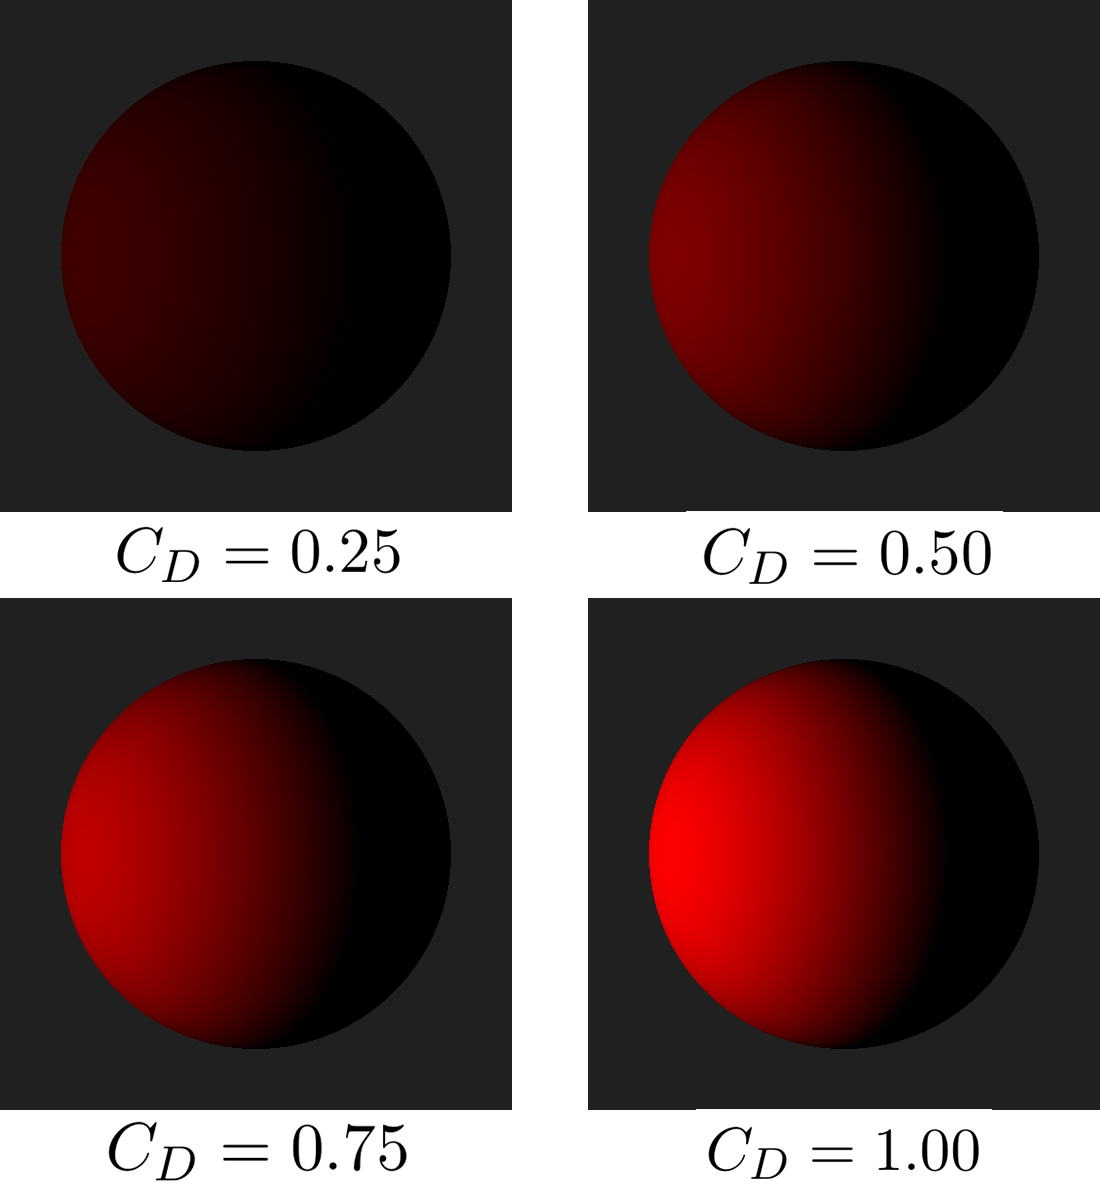
\includegraphics[width=0.5\textwidth]{img/rt/differentDiffuse.png}}

	\caption{Le rendu de la même sphère pour différents coefficients de diffusion $C_D$ de l'objet. On devine la position de la source lumineuse à gauche.}
	\label{differentDiffuse}
\end{figure}
\FloatBarrier

La dernière composante est la spéculaire. Elle est responsable des points de reflets qu'on peut voir dans la vraie vie sur des objets en plastique notamment. L'idée de son fonctionnement est la suivante:\\
Plus le rayon de lumière qui frappe l'objet en un point donné est réfléchi droit sur la caméra, plus l'intensité spéculaire en ce point est importante. Le calcul de la spécularité:

\begin{center}
	$Specularite = I_S = C_S*(\overrightarrow{d_{ray}}\cdot\overrightarrow{R_{light}})^\alpha$
\end{center}
$C_S$ étant le coefficient d'intensité spéculaire de l'objet,\\
$\overrightarrow{d_{ray}}$ la direction du rayon qui a intersecté l'objet,\\
$\overrightarrow{R_{light}}$ la direction du rayon de lumière entre la source de lumière et le point d'intersection s'il est parfaitement réfléchi (voir la partie \ref{reflexions} sur les réflexions) par rapport à la surface de l'objet,\\
$\alpha$ la "brillance" de l'objet. Plus ce paramètre est élevé plus les tâches spéculaires seront petites. L'objet paraîtra plus brillant.

D'une façon analogue au fonctionnement de la composante diffuse, plus le produit scalaire des vecteurs $\overrightarrow{R_{light}}$ et $\overrightarrow{d_{ray}}$ se rapproche de 1, plus l'intensité de la spécularité sera forte.\\
Le paramètre alpha permet quant à lui de jouer sur la taille des tâches spéculaires. En effet, on observe sur la \figurename~\ref{differentSpecular}, pour $C_S = 1$ et $\alpha = 10$, que la tâche spéculaire est moins intense sur ses bords qu'en son centre.\\
On peut grossièrement estimer que l'intensité lumineuse de la spécularité $I_S$ aux bords de la tâche spéculaire est comprise entre 0.5 et 1: $0.5 \leqslant I_S \leqslant 1$.\\
Ainsi $I_S$, décroîtra rapidement vers 0 lorsque élevée à la puissance $\alpha$. A contrario, $I_S$ se rapprochant de 1 au centre de la tâche lumineuse, la décroissance vers 0 sera plus lente, bien que tout à fait présente comme en témoigne la \figurename~\ref{differentSpecular} aux paramètres $C_S = 1$ et $\alpha = 512$.

\begin{figure}[h!]
	\adjustbox{center}{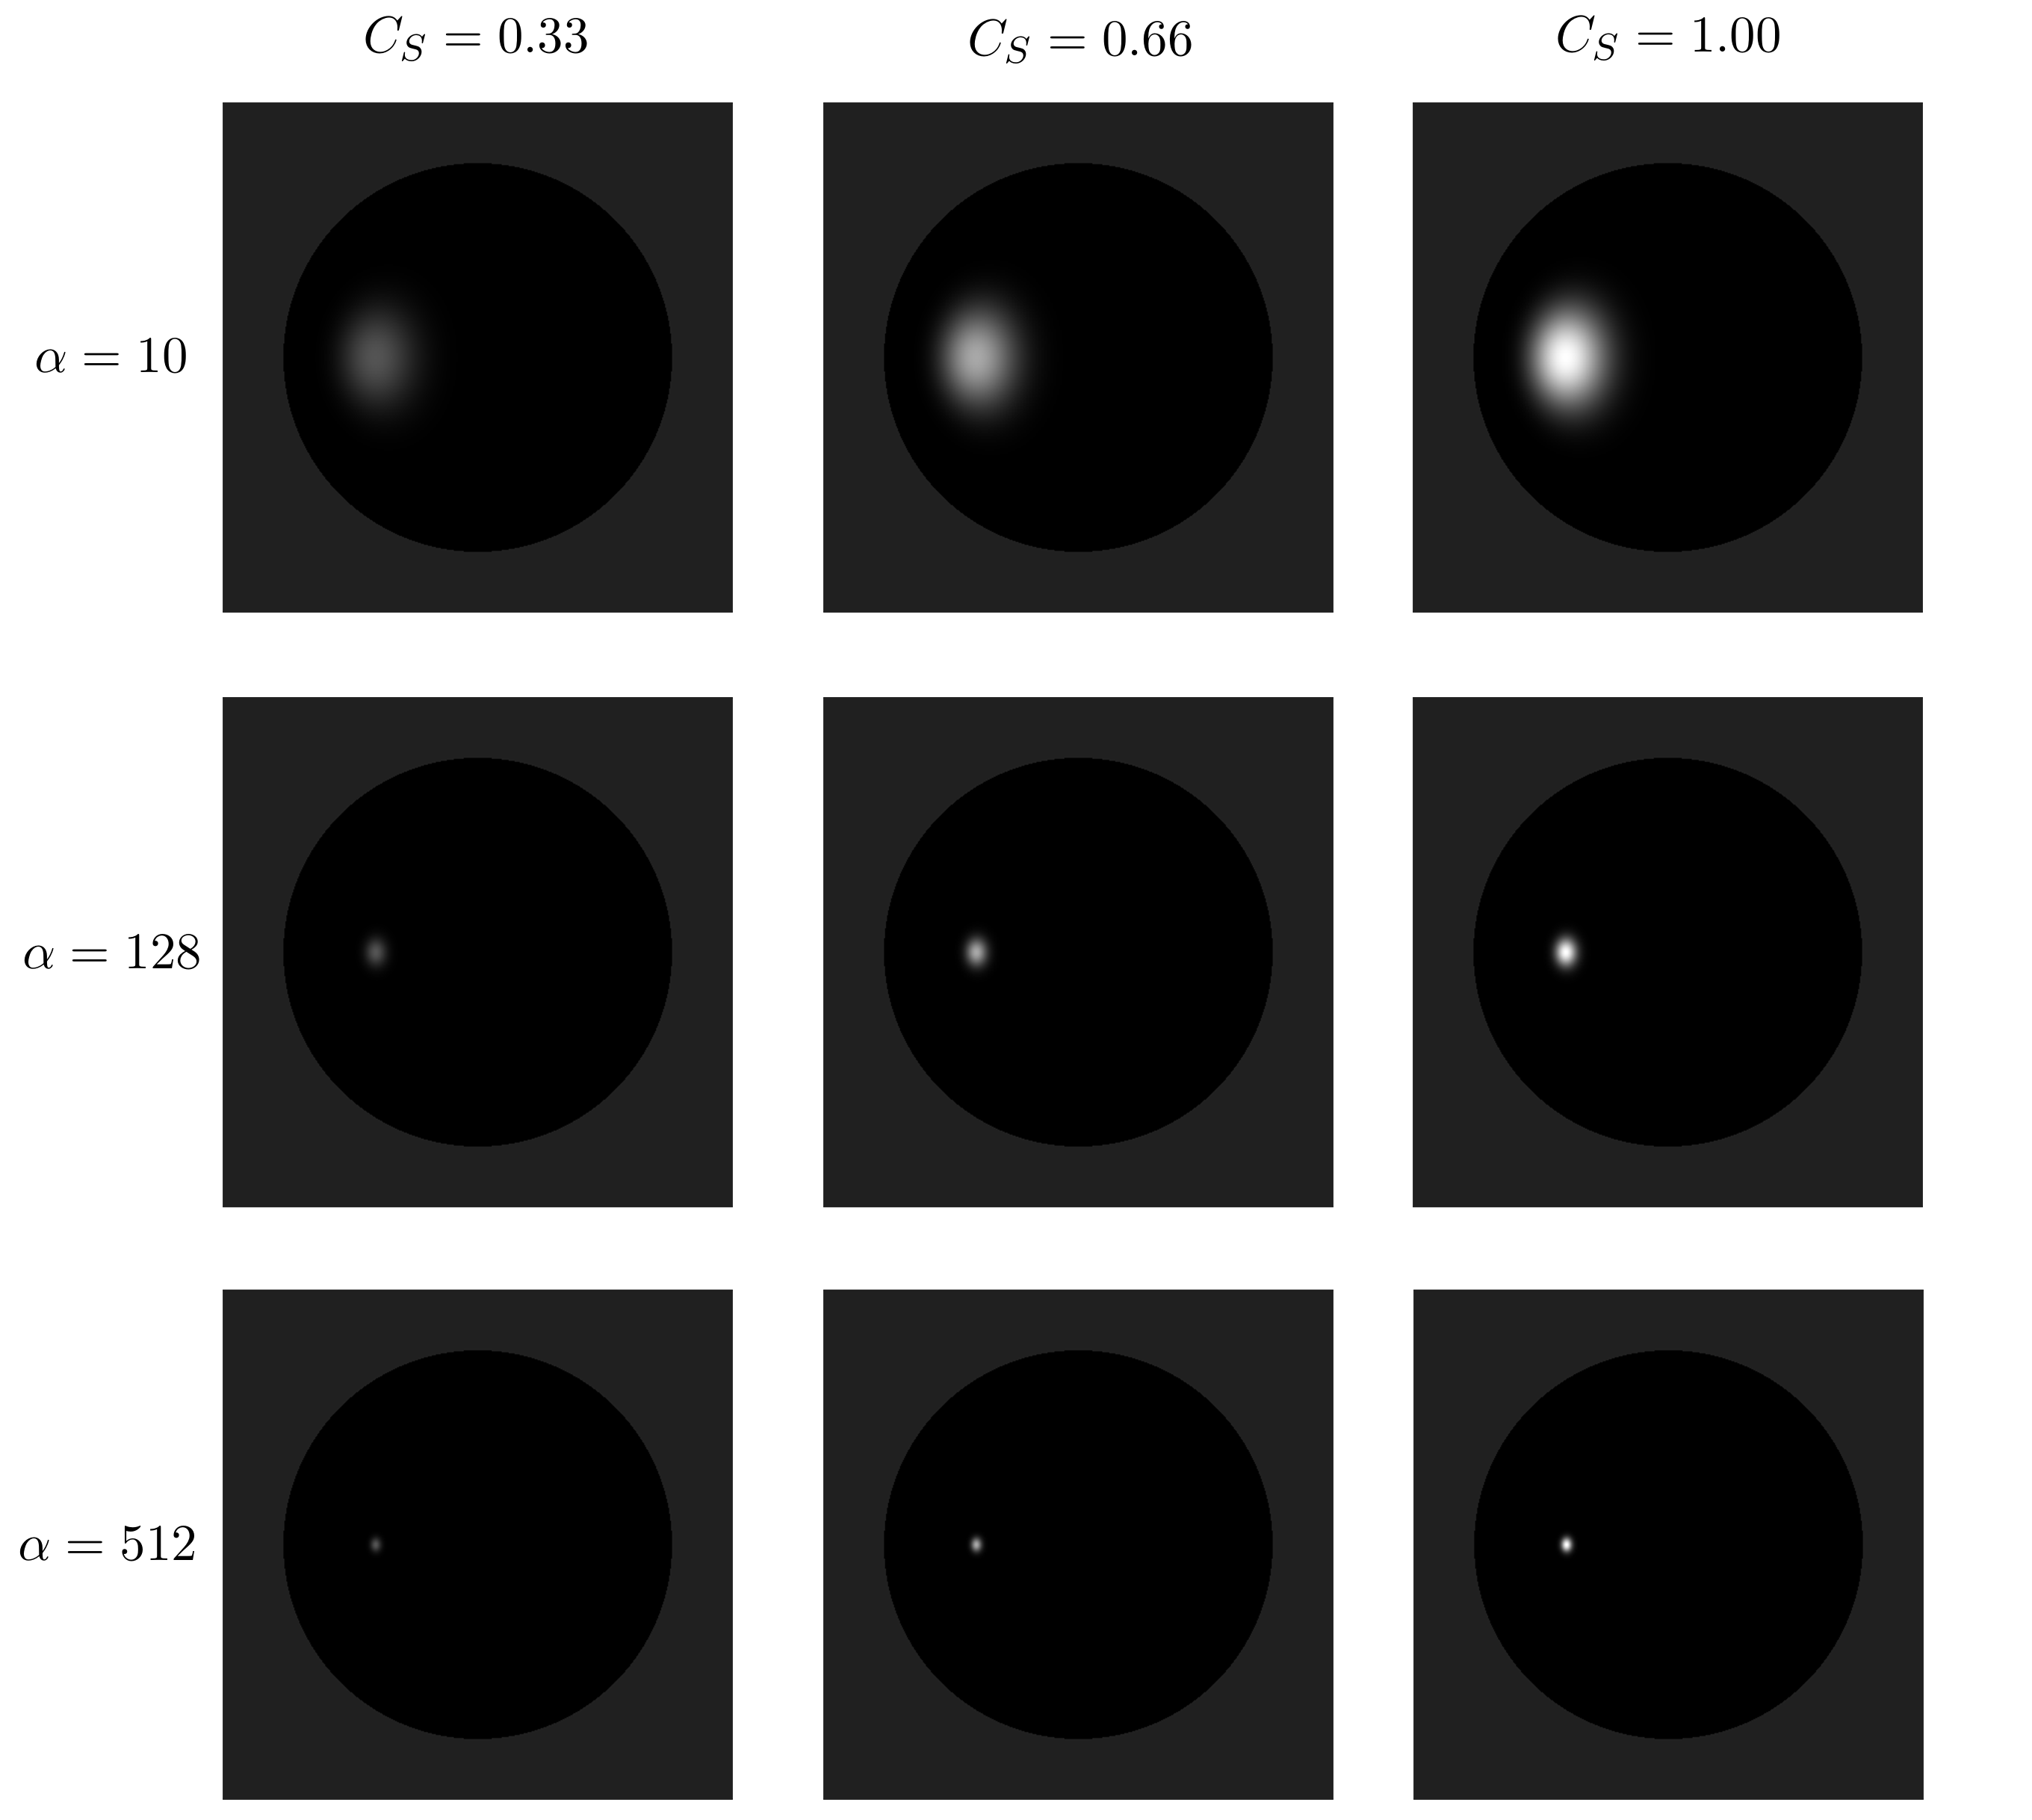
\includegraphics[width=0.8\textwidth]{img/rt/differentSpecular.png}}

	\caption{Le rendu de la même sphère pour différents coefficients de spécularité $C_S$ de l'objet et différentes valeurs du paramètre $\alpha$. La source lumineuse est à gauche.}
	\label{differentSpecular}
\end{figure}
\FloatBarrier

Les trois composantes de l'ombrage de Phong étant maintenant calculées, nous pouvons calculer l'intensité lumineuse totale en un pixel $P_{(x, y)}$ donné de l'image:
\begin{itemize}
	\item{Si le rayon passant par ce pixel n'intersecte rien, la couleur renvoyée est celle du fond de la scène}
	\item{Si le rayon intersecte un objet, la couleur renvoyée est:}
\end{itemize}
\begin{center}
$C_{P(x, y)} = C_O * IntensitePhong = C_O*(I_A + I_D + I_S)$
\end{center}
$C_O$ étant la couleur de l'objet,\\
$I_A, I_D, I_S$ sont les intensités ambiantes, diffuses et spéculaires présentées précédemment.

Pour la même sphère et la même source de lumière, nous obtenons alors:

\begin{figure}[h!]
	\adjustbox{center}{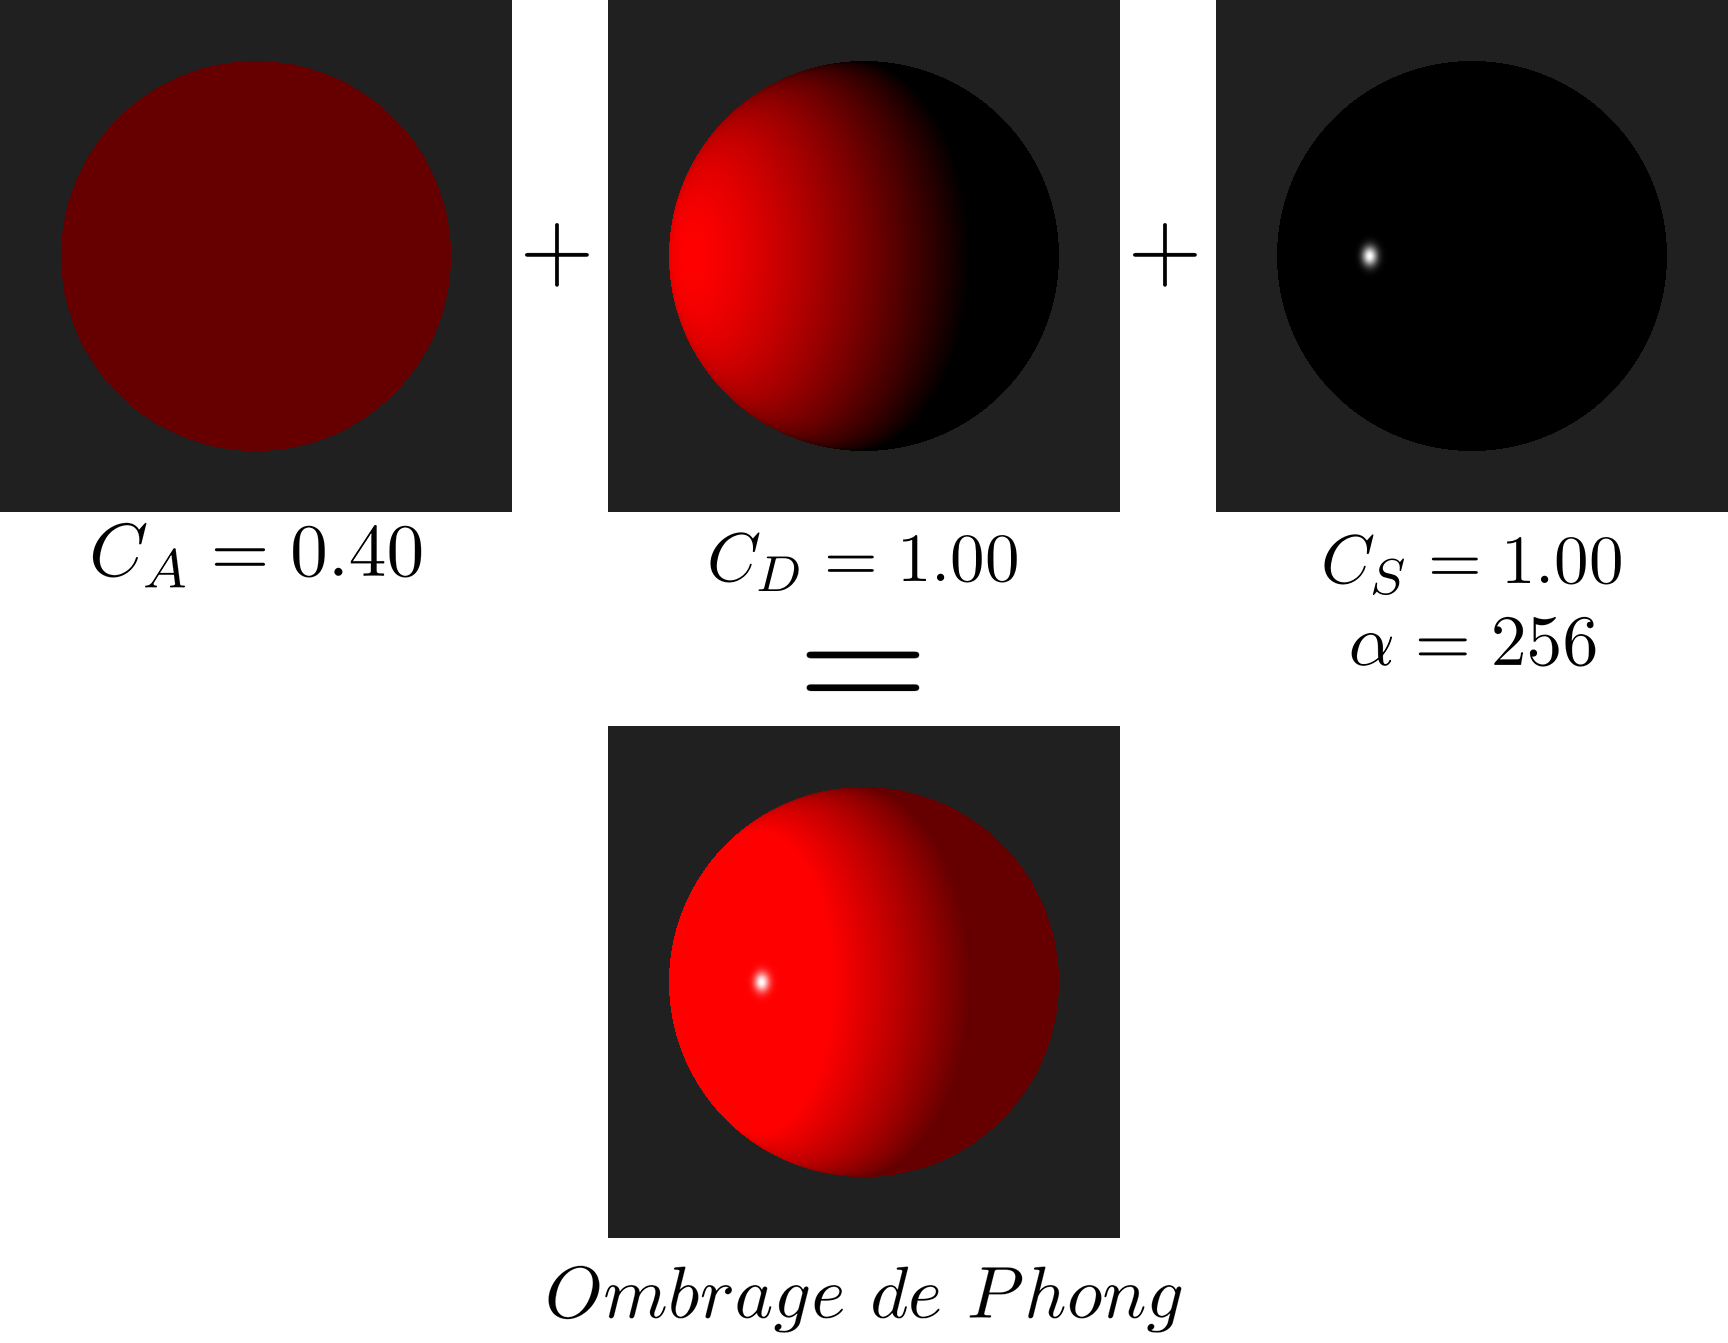
\includegraphics[width=0.75\textwidth]{img/rt/phongAddition.png}}

	\caption{Rendu final de la sphère en additionnant toutes les composantes de l'ombrage de Phong}
	\label{finalPhong}
\end{figure}
\FloatBarrier

\subsubsection{Les ombres}

Afin de rajouter un degré de réalisme au rendu, nous nous proposons de rajouter des ombres. Le principe est simple: pour chaque rayon tiré depuis la caméra, on se place au point d'intersection trouvé par le rayon avec un objet de l'environnement. Depuis ce point, on tire un autre rayon directement en direction de la source de lumière. Si ce nouveau rayon vient à intersecter quelque chose sur son chemin à la lumière, cela veut dire que nous sommes dans l'ombre. Quelque chose bloque l'accès direct à la lumière. La couleur du pixel sera alors seulement la partie ambiante de l'objet premièrement intersecté. Si ce deuxième rayon n'intersecte rien, nous ne sommes pas dans l'ombre et nous pouvons calculer l'intensité lumineuse en utilisant l'ombrage de Phong vu en partie \ref{ombragePhong}. De part leur nature, on appelle ces rayons secondaires des "shadow ray".

\begin{figure}[h!]
	\adjustbox{center}{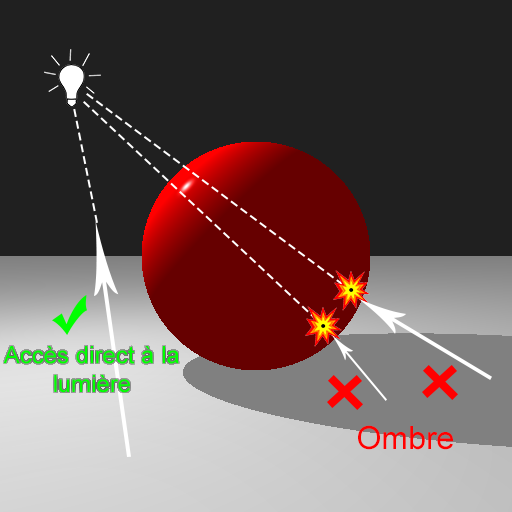
\includegraphics[width=0.5\textwidth]{img/rt/ombresSchema.png}}

	\caption{Des points d'intersection ont été trouvés avec le plan derrière la sphère. Les shadow-ray tirés depuis ces points d'intersection ne peuvent pas accéder directement à la lumière. C'est une zone d'ombre.}
	\label{ombresSchema}
\end{figure}
\FloatBarrier

L'algorithme de calcul de la couleur de chacun des pixels peut donc être adapté pour tenir compte des ces nouvelles ombres:

\begin{algorithm}[H]
	\KwIn{$x, y$ les coordonnées du pixel dont on souhaite calculer la couleur}
	\KwOut{$C_P$, la couleur du pixel\\\hfill\\}
	
	coord$_{(x, y)} \gets$ conversionPixelScene(x, y)\\
	cameraRay $\gets$ $Rayon(camera, coord_{(x, y)})$\\
	\If{cameraRay.intersects(objetScene)}
	{
		intersectedObject $\gets$ objet intersecté par $cameraRay$\\\hfill\\
		shadowRay $\gets Rayon(pointIntersection, lumiere)$\\
		\If(\tcp*[h]{Le point d'intersection est dans l'ombre}){shadowRay.intersects(objetScene)}
		{
			\Return{$Color_{intersectedObject} * I_A$}
		}
		\Else(\tcp*[h]{Nous ne sommes pas dans l'ombre})
		{
			\Return{phongShading(pointIntersection)}
		}
	}
	\Else
	{
		\Return{backgroundColor}
	}

	\caption{Algorithme retournant la couleur d'un pixel en fonction du fait qu'il soit dans l'ombre ou non - computeShadow}
	\label{algoOmbres}
\end{algorithm}

\subsubsection{Les réflexions}
\label{reflexions}

Jusqu'alors, notre algorithme n'a été capable de rendre que des objets dont le matériau est matte. La spécularité peut éventuellement donner un effet de brillance mais ce n'est qu'une impression. En ajoutant des matériaux réflexifs, nous pourrons créer des objets qui réfléchissent la lumière à la façon d'un miroir ou des objets à l'aspect métallique. Le principe derrière le calcul des réflexions est le suivant:
\begin{itemize}
	\item{Si le camera-ray lancé intersecte un objet qui n'est pas réfléchissant, calculer sa couleur avec l'ombrage de Phong comme vu précédemment.}
	\item{Si le rayon intersecte un objet réfléchissant, calculer la direction du rayon réfléchi et lancer un nouveau rayon dans cette direction de façon récursive. La couleur renvoyée sera alors la dernière chose que touche le rayon (un objet non réflexif ou le fond de la scène)}
\end{itemize}
La direction d'un rayon parfaitement réfléchi peut se calculer grâce au rayon incident $I$ ainsi que grâce à la normale de la surface au point d'intersection $N$:

\begin{figure}[h!]
	\adjustbox{center}{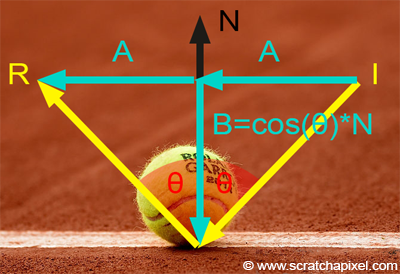
\includegraphics[width=0.5\textwidth]{img/rt/reflectionVector.png}}

	\caption{On peut calculer le rayon réfléchi à partir du rayon incident et de la normale. \textbf{Source: scratchapixel.com} \cite{scratchapixel}}
	\label{reflectionCalcul}
\end{figure}
\FloatBarrier

La \figurename\ \ref{reflectionCalcul} nous montre qu'une balle de tennis (jouant le rôle d'un rayon) rebondira avec un angle de sortie $\theta$ égal à son angle d'arrivée ($\theta$) par rapport au sol. Le principe est le même avec les rayons. Par construction géométrique, on obtient la direction du rayon réfléchi:

\begin{center}
	$\overrightarrow{R} = \overrightarrow{I} - (\overrightarrow{N}\cdot \overrightarrow{I})*\overrightarrow{N}*2$
\end{center}

Il ne reste plus, pour calculer la couleur de la réflexion, qu'à prendre en compte le coefficient de réflexion $C_R$ du matériau. On obtient alors l'algorithme:

\begin{algorithm}[H]
	\DontPrintSemicolon
	\KwIn{$\overrightarrow{R}$ le rayon incident, $depth$ la profondeur actuelle}
	\KwOut{La couleur du pixel $P_{(x, y)}$ par lequel est passé le camera-ray initial\\\hfill\\}

	\If(\tcp*[h]{La profondeur de récursion maximale a été atteinte}){depth == 0}
	{
		\Return{backgroundColor}
	}
	\hfill\\

	\If(\tcp*[h]{On vérifie si on a intersecté quelque chose}){$\overrightarrow{R}$.intersects(objetsScene)}
	{
		intersectedObject $\gets$ objet intersecté par $\overrightarrow{R}$\\\hfill\\

		\If(\tcp*[h]{Si l'objet intersecté est réfléchissant}){intersectedObject.isReflexive()}
		{
			$\overrightarrow{R_{reflect}} \gets$ computeReflectedDirection($\overrightarrow{R}$, $\overrightarrow{N}$)\\\hfill\\

			\Return{$C_R*$computeReflection($\overrightarrow{R_{reflect}}$, depth - 1)}{\tcp*[h]{On effectue un appel récursif pour relancer un rayon}}
		}
		\Else(\tcp*[h]{L'objet n'est pas réfléchissant, on va simplement retourner son ombrage de Phong})
		{
			\Return{phongShading()}
		}
	}
	\Else
	{
		\Return{backgroundColor}
	}

	\caption{Algorithme de calcul des réflexions pour des objets non colorés - computeReflection}
	\label{algoReflections}
\end{algorithm}

Cet algorithme suppose que l'objet n'est pas coloré et donc qu'il renvoie les rayons tels quels. Dans le cas d'un objet métallique cependant, un lingot d'or par exemple, la réflexion sera colorée par la couleur du matériau. La méthode n'est pas présentée ici car il ne s'agit que de montrer le principe des réflexions.

\begin{figure}[!h]
	\adjustbox{center}{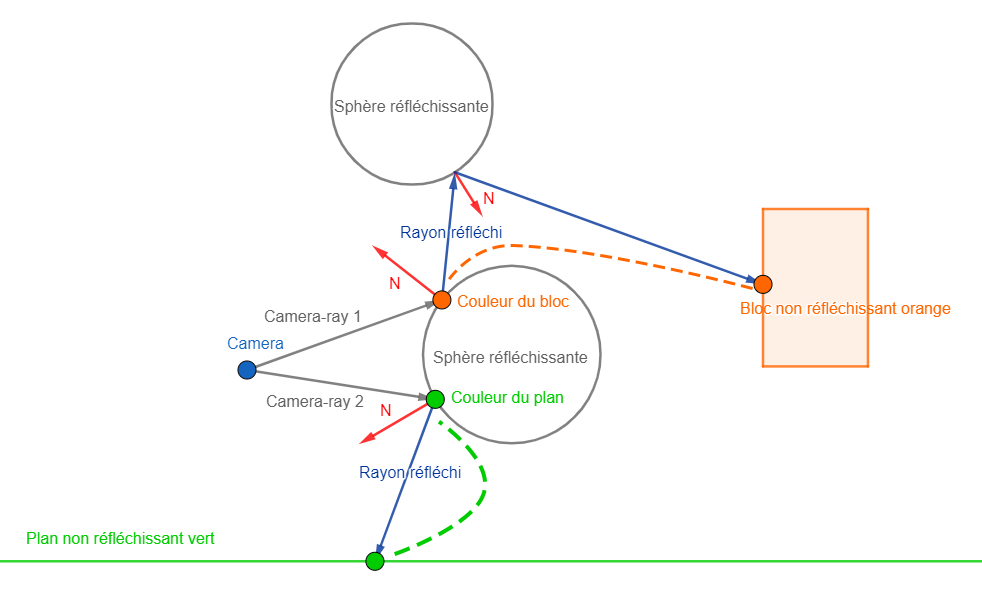
\includegraphics[width=1.1\textwidth]{img/rt/reflectionsSchema.png}}

	\caption{Exemple de rebonds successifs des rayons jusqu'à un objet non réfléchissant}
	\label{reflectionsSchema}
\end{figure}
\FloatBarrier

La \figurename\ \ref{reflectionsDemo} montre un résultat que l'ont peut obtenir avec deux sphères réflexives (une au centre et une à sa droite), plusieures sphères mattes ainsi qu'un plan:

\begin{figure}[h!]
	\adjustbox{center}{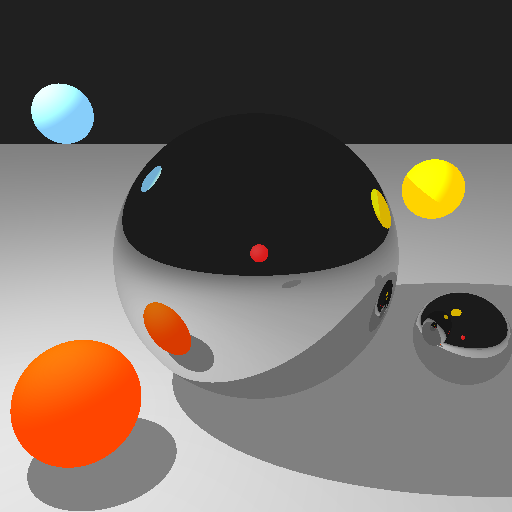
\includegraphics[width=0.5\textwidth]{img/rt/reflectionsDemo.png}}

	\caption{On peut voir une sphère rouge derrière la caméra grâce à la reflexion de la sphère centrale. Les coefficients de réflexion ont été fixés à 0.8 pour ce rendu.}
	\label{reflectionsDemo}
\end{figure}
\FloatBarrier

La prochaine étape consistera à ajouter le support des objets transparents en implémentant un système de réfraction des rayons.
\subsubsection{Les réfractions}

\subsection{Les mouvements de caméra}

Notre projet nous permet de déplacer la caméra dans la scène et de recalculer en temps réel les images en accord avec la position de la caméra. Cependant, déplacer la caméra ne se résume pas à changer la position de la caméra. Divers calculs vont en effet être nécessaires afin que le rendu soit fidèle à la nouvelle position de la caméra.
\subsubsection{Les mouvements de translation}
Notre caméra est capable de deux types de mouvement. Les translations et les rotations (partie \ref{rotationsCamera}). Nous allons voir dans cette partie comment nous pouvons déplacer l'origine de la caméra sans changer sa direction de regard (rotation de la caméra).

Par convention, la position de base de la caméra dans la scène est $P=(0, 0, 0)$. Nous avons également vu dans la partie \ref{conversionCamera} (voir \figurename\ \ref{repreCamRayon}) que le plan de la caméra se trouvait à 1 unité de distance. Par conséquent, dans le cas où la caméra est toujours dans sa position d'origine, les coordonnées d'un pixel $PixelWorld$ exprimées dans l'espace de la scène seront de la forme:

\begin{center}
	$PixelWorld = (x, y, -1)$
\end{center}

Si on déplace la caméra de 4 unité dans le sens de l'axe X, les coordonnées du pixel dans l'espace de la scène deviennent:

\begin{center}
	$PixelWorld = (x + 4, y, -1)$
\end{center}

De même, en déplaçant, la caméra de 3 unité dans le sens de l'axe Y en plus de la translation précédente, on obtient:

\begin{center}
	$PixelWorld = (x + 4, y + 3, -1)$
\end{center}

\begin{figure}[h!]
	\adjustbox{center}{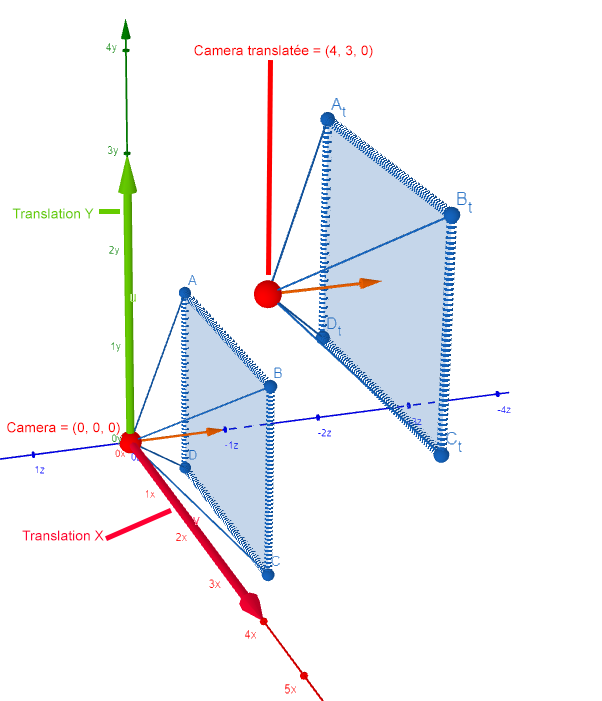
\includegraphics[width=0.9\textwidth]{img/rt/translationCamera.png}}
	
	\caption{Représentation de la translation de la caméra par les vecteurs $T_X = (4, 0, 0)$ et $T_Y = (0, 3, 0)$}
	\label{translationCameraFigure}
\end{figure}
\FloatBarrier

Nous remarquons qu'il suffit alors d'appliquer la même translation que nous avons appliqué à la caméra aux coordonnées des pixels dans l'espace de la scène. Les rayons que nous lancerons depuis la caméra auront alors pour origine la position de la caméra translatée et comme point de direction les nouvelles coordonnées des pixels translatés.\\
Plus formellement, pour une translation $\overrightarrow{u} = (a, b, c)$, $P_T$ la position de la caméra translatée et $PixelWorld = (x, y, -1)$ les coordonnées du pixel visé exprimées dans l'espace de la scène:

\begin{center}
	$Rayon_T = (P_T, (x + a, y + b, -1 + c))$
\end{center}

\subsubsection{Les mouvements de rotation}

La caméra pouvant maintenant être translatée, il reste à implémenter les rotations. Pour ce faire, nous considérerons 3 caractéristiques de la caméra:
\begin{itemize}
	\item{Sa direction de regard $\overrightarrow{d} = (0, 0, -1)$ par défaut}
	\item{Son angle de rotation horizontal. 0 par défaut}
	\item{Son angle de rotation vertical. 0 par défaut}
\end{itemize}
\hfill\\
A l'aide de ces 3 caractéristiques, nous pouvons définir deux types de rotation:
\begin{itemize}
	\item{Les rotations horizontales}
	\item{Les rotations verticales}
\end{itemize}

Une rotation horizontale est une rotation d'angle $\alpha$ autour de l'axe y. Une rotation verticale est une rotation d'angle $\beta$ autour de l'axe x:
Ci-dessous, ce à quoi ressemble une rotation autour de l'axe Y de la caméra. Une rotation horizontale donc.

\begin{figure}[h!]
	\adjustbox{center}{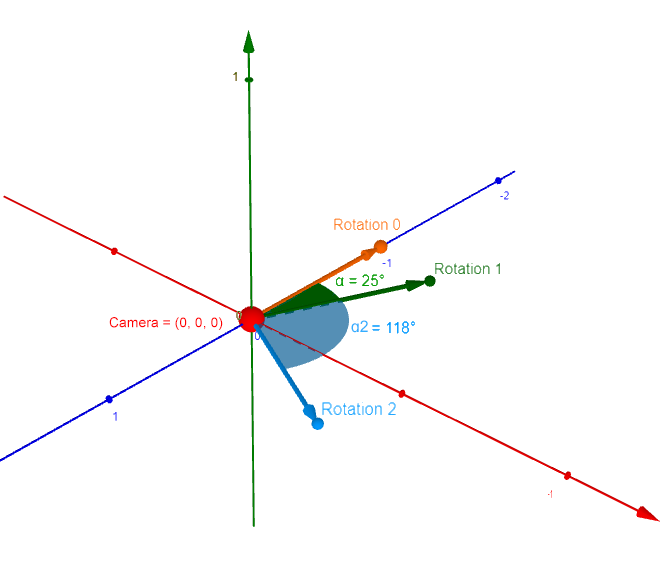
\includegraphics[width=\textwidth]{img/rt/rotationCameraY.png}}

	\caption{Exemples de plusieures rotations horizontales de la caméra}
	\label{rotationCameraY}
\end{figure}
\FloatBarrier

De même pour les rotations verticales autour de l'axe X:

\begin{figure}[h!]
	\adjustbox{center}{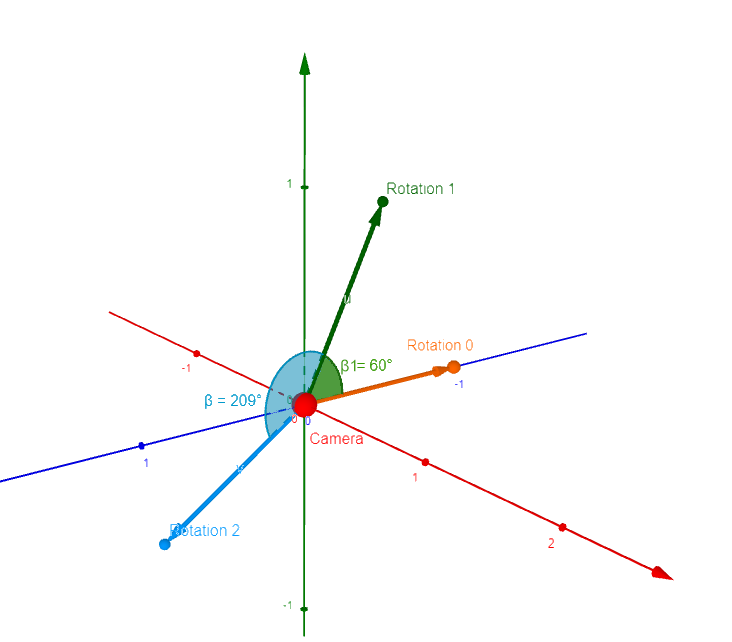
\includegraphics[width=\textwidth]{img/rt/rotationCameraX.png}}

	\caption{Exemples de plusieures rotations verticales de la caméra}
	\label{rotationCameraX}
\end{figure}
\FloatBarrier

En combinant et les rotations verticales et les rotations horizontales, on obtient ainsi n'importe quelle rotation dans l'espace. Cela nous permet donc, de regarder n'importe quel point de la scène avec la caméra. La seule exception étant les rotations autour de l'axe Z qui ne sont pas supportées par notre RayTracer. Il s'agit de rotations qui permettraient de faire passer le sol au plafond et le ciel au sol par exemple. Une métaphore culinaire pour imager ces rotations autour de l'axe Z seraient un poulet rôti sur une broche. La broche étant l'axe Z autour duquel tourne le poulet, la caméra.

\subsubsection{La matrice de transformation CTWMatrix}
\label{rotationsCamera}

Afin de ne pas manipuler les deux rotations et la translation de la caméra individuellement, nous allons utiliser une matrice de transformation. Cette matrice nous permettra d'effectuer toutes les transformations voulues en une opération. Elle porte le nom de CTWMatrix, Camera To World Matrix. En effet, c'est une matrice de passage entre la base de l'espace vectoriel de la caméra et la base de l'espace vectoriel du monde. On peut ainsi l'utiliser pour convertir les coordonnées des points exprimées dans l'espace de la caméra en coordonnées exprimées dans l'espace du monde. C'est exactement ce dont nous avons besoin pour les rotations de la caméra et les translations.\\
Pour construire une telle matrice, nous utiliserons tout d'abord deux matrices de rotation:
\begin{center}
	$R_Y =
	\begin{pmatrix}
		cos(\alpha) & 0 & sin(\alpha)\\
		0 & 1 & 0\\
		-sin(\alpha) & 0 & cos(\alpha)
	\end{pmatrix}
	$ ;
	$R_X = 
	\begin{pmatrix}
		1 & 0 & 0\\
		0 & cos(\beta) & -sin(\beta)\\
		0 & sin(\beta) & cos(\beta)
	\end{pmatrix}
	$\\
	\textbf{Source: wikipedia} \cite{wikipediaRotationMatrices}
\end{center}

$(MR_{3x3}, \cdot)$ l'ensemble des matrices de rotation de taille 3x3 muni de la multiplication usuelle des matrices est un groupe. Ainsi, $R_Y\cdot R_X$ est une matrice de rotation qui de plus, combine les rotations de $R_Y$ et de $R_X$. Cependant ce n'est pas un groupe abélien et en général, $R_Y\cdot R_X \ne R_X\cdot R_Y$. On en déduit qu'une rotation autour de l'axe X suivie d'une rotation autour de l'axe Y ne donne pas la même rotation finale que la même rotation autour de l'axe Y suivie de la même rotation autour de l'axe X. Il va donc falloir choisir un ordre de rotation autour des axes. Nous avons choisi de tourner autour de l'axe Y en premier puis autour de l'axe X.\\
Si $R_{YX} = R_Y\cdot R_X$, il ne manque plus qu'à prendre en compte la transformation de translation. Comme vu précédemment, il suffit, pour translater un point, d'ajouter coordonnées à coordonnées le vecteur de translation et le point à translater. Une matrice de translation est alors de la forme:

\begin{center}
	$T_{\overrightarrow{u}} =
	\begin{pmatrix}
		1 & 0 & 0\\
		0 & 1 & 0\\
		0 & 0 & 1\\
		a & b & c
	\end{pmatrix}
	$
\end{center}
avec $\overrightarrow{u} = (a, b, c)$ le vecteur de translation.\\
Pour combiner notre matrice de rotation $R_{YX}$ avec notre matrice de translation $T_{\overrightarrow{u}}$, on ajoute la ligne $(a\ b\ c)$ à notre matrice $R_{YX}$ et on obtient:

\begin{center}
	$CTWMatrix =
	\begin{pmatrix}
		R_{YX_{0, 0}} & R_{YX_{0, 1}}  & R_{YX_{0, 2}}\\
		R_{YX_{1, 0}} & R_{YX_{1, 1}}  & R_{YX_{1, 2}}\\
		R_{YX_{2, 0}} & R_{YX_{2, 1}}  & R_{YX_{2, 2}}\\
		a & b & c
	\end{pmatrix}
	$
\end{center}
Cette matrice combine alors les rotations et la translation dont nous avons besoin. Multiplier un point par cette matrice fera alors passer les coordonnées de ce point dans l'espace de la scène. Les coordonnées de nos points étant cependant de dimension 3 et notre matrice étant de taille 4x3, on peut tout de même multiplier un point avec la CTWMatrix en ajouter une 4ème coordonnée à notre point $P(x, y, z)$ :
\begin{center}
	$P = (x, y, z, 1)$
\end{center}
Cette 4ème coordonnée ne sert que pour les calculs et doit être ignorée dans le point résultant de la multiplication avec la matrice.

\begin{center}
	$P(x, y , z) \longrightarrow P(x, y, z, 1)$\\
	$P \cdot CTWMatrix = P_{convert}(x', y', z', w) \longrightarrow P(x', y', z')$
\end{center}
Notre point dont les coordonées ont été converties est alors $P(x', y', z')$.

\subsection{Le multithreading}
\subsubsection{Organisation et mise en place}

Les algorithmes de Ray Tracing sont capables de générer des images réalistes mais sont, en contrepartie, assez lents à exécuter. Un avantage cependant de ces algorithmes est que chaque pixel est calculé indépendamment des autres. Il n'y a pas besoin d'attendre que le "pixel 1" soit calculé pour pouvoir calculer le "pixel 2". Tous les pixels sont indépendants les uns des autres. Cela fait donc de ces algorithmes des cibles parfaites pour la parallélisation des calculs. Dans le cas de notre implémentation, elle est executée par le processeur de l'ordinateur. Nativement, notre programme n'était pas parallélisé et seul un des processeurs du CPU de la machine s'attelait à la tâche. L'idée était alors d'utiliser toute la puissance du CPU mise à disposition pour accélérer les temps de rendu. Pour ce faire, l'image à rendre est tout d'abord découpée en tuiles:

\begin{figure}[h!]
	\adjustbox{center}{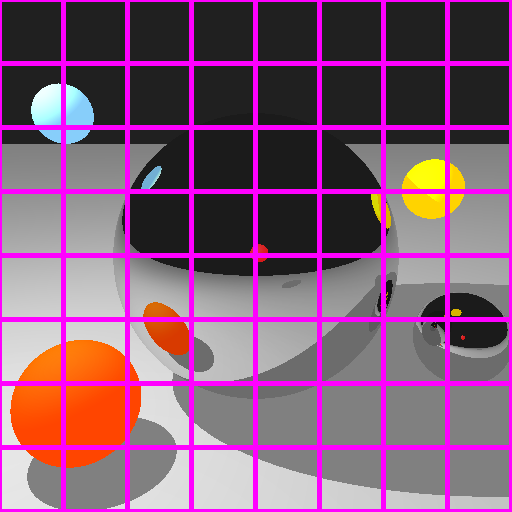
\includegraphics[width=0.5\textwidth]{img/rt/grilleMultithreading.png}}

	\caption{L'image que l'on veut rendre est découpée en tuiles}
	\label{grilleMultithreading}
\end{figure}
\FloatBarrier

Afin de faciliter la gestion du multithreading, différentes classes vont être utilisées comme montré dans la \figurename\ \ref{packageMultithreading}. On utilisera les classes \textit{TileTask}, \textit{ThreadsTaskList} ainsi que \textit{TileThread}. Pour chaque tuile dont est composée l'image à rendre, nous allons créer la TileTask lui correspondant, définissant les dimensions de cette tuile:
\begin{itemize}
	\item {Les positions de départ de la tuile x et y}
	\item {Les positions de fin de la tuile x et y}
\end{itemize}
\hfill\\
Dans le cas de la \figurename\ \ref{grilleMultithreading}, l'image à rendre a été découpée en 8x8 = 64 tuiles ou (tasks). Chacune de ces \textit{TileTask} alors créée va être ajoutée à une \textit{ThreadsTaskList} créée en amont (voir \figurename\ \ref{packageMultithreading}). Cette \textit{ThreadsTaskList} gardera compte de combien de tâches (tuiles) sont à rendre au total, combien de tâches restent à rendre et combien de tâches ont été rendues. Comme son nom l'indique, cette classe disposera aussi de la liste des tâches elle même.

\begin{figure}[h!]
	\adjustbox{center}{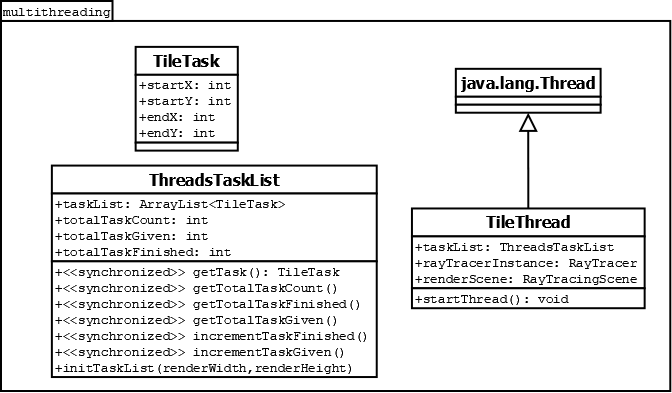
\includegraphics[width=0.85\textwidth]{diagrammes/package_multithreading.png}}

	\caption{Package multithreading}
	\label{packageMultithreading}
\end{figure}
\FloatBarrier

Maintenant que nous avons notre liste de tâches prête, la prochaine étape est celle de la création des threads, de la distribution et du calcul des tâches. Nous allons pour cela utiliser la dernière classe du package multithreading, \textit{TileThread}. Cette classe permet de représenter des threads de calcul du ray tracer. Chaque \textit{TileThread} créé gardera une référence sur la liste de tâches à calculer ainsi que sur la scène de rendu et sur l'instance du Ray Tracer.

\begin{algorithm}[H]
	\KwIn{tskList une instance de ThreadsTaskList initialisée avec les tâches créées au préalable,\\
		RTInst l'instance du Ray Tracer,\\
		scene la scène contenant les objets à rendre,\\
		threadCount le nombre de thread voulu pour le rendu\hfill\\}
	
	\For {$i \in \llbracket 1; threadCount \llbracket$}
	{
		thread = creerThread(TileThread(tskList, RTInst, scene))

		demarrer(thread)
	}\hfill\\

	\While(\tcp*[h]{Tant qu'il reste des tâches à calculer}){$tskList.totalTaskFinished < taskList.totalTaskCount$}
	{
		computeTask(tskList)
	}

	\caption{Algorithme gérant la création des threads}
	\label{creationThreads}
\end{algorithm}
\hfill\\
L'algorithme \ref{creationThreads} qui crée les threads de calculs présente une subtilité. $threadCount-1$ threads sont créés et non pas $threadCount$. En effet, le thread principal va lui aussi s'atteler à la tâche, c'est un thread déjà créé par le lancement du programme lui même. On crée donc un thread de moins. Après la création des threads, une boucle while permet de donner au thread principal autant de tâche qu'il en reste à calculer (pendant que les autres threads calculent aussi leurs tâches en parallèle). Ainsi, lorsque la condition de la boucle while ne sera plus vérifiée, cela signifiera que toutes les tâches ont été calculées.Le thread principal pourra sortir de la boucle et le rendu pourra être affiché. Voyons maintenant comment fonctionne la méthode \textit{computeTask} utilisée dans l'algorithme présenté précédemment.

\begin{algorithm}[H]
	\KwIn{\textit{renderScene}, la scène dont on veut faire le rendu,\\
		\textit{taskList}, la liste des tâches que les threads vont devoir calculer\\\hfill\\}

	\lstinputlisting[language=Java]{code/computeTask.java}
	
	\caption{Java - Méthode de gestion des calculs des tâches}
	\label{computeTask}
\end{algorithm}
\hfill\\
Cette méthode sera utilisée par tous les threads ayant été créé. Elle est destinée à donner les tâches aux threads tant qu'il en reste à calculer. A l'entrée de la méthode, on vérifie si toutes les tâches ont déjà été données à calculer. Si c'est le cas, on retourne false, indiquant qu'il n'y a plus de tâches à donner aux threads. S'il reste des tâches à calculer, on récupère la prochaine tâche et on incrémente la variable qui tient compte du nombre de tâches qui ont été données à calculer. On calcule ensuite la tuile correspondant à la tâche et on incrémente le nombre de tâche qui ont été calculées. On retourne alors true puisque le thread a calculé une tâche avec succès, il peut y en avoir d'autre à calculer. L'utilisation des blocs \color{javapurple}{\textbf{synchronized}} \color{black} de Java est justifiée pour éviter la concurrence des threads sur les variables partagées entre tous les threads de calcul. En effet, les variables totalTaskCount, totalTaskGiven et totalTaskFinished sont réécrites par tous les threads, potentiellement simultanément. Les blocs \color{javapurple}{\textbf{synchronized}}\color{black}\ sont alors nécessaires pour éviter de nombreux problèmes.

La méthode \textit{demarrer(thread)} permet de lancer le thread après l'avoir créé. Le thread va alors exécuter le code de sa méthode de départ:

\begin{algorithm}[H]
	\lstinputlisting[language=Java]{code/demarrerThread.java}

	\caption{Point de départ des threads, appelé par \textit{demarrer}}
	\label{methodeDemarrer}
\end{algorithm}
computeTask retournant false quand il n'y a plus de tâche à effectuer et true sinon, on peut simplement mettre l'appel de la méthode dans une boucle infinie. Cela aura pour effet de donner des tâches à calculer aux threads tant qu'il y en a. Dès que toutes les tâches auront été données, computeTask retournera false, le thread quittera la boucle et pourra être terminé.

\subsubsection{Les performances}

Le but de notre parallélisation étant d'accroître les performances du ray tracer, nous présentons dans cette section les résultats en termes de performances de notre implémentation.\\
Nous comparerons les temps de rendu par image pour différentes résolutions et différents nombre de threads. L'image sera toujours découpée en $nbThread^2$ tuiles.

\begin{center}
	\begin{tabular}{|c|c|c|c|c|}
		\hline
		\backslashbox{Nombre de thread}{Résolution de rendu} & 128*128 & 256*256 & 512*512 & 1280*720\\
		\hline
		1 & 5.01ms & 18.39ms & 72.87ms & 240.54ms\\
		2 & 2.63ms & 9.81ms & 38.49ms & 126.79ms\\
		4 & 1.64ms & 5.54ms & 23.02ms & 78.42ms\\
		8 & 1.46ms & 4.47ms & 16.72ms & 55.58ms\\
		\hline
	\end{tabular}
\end{center}
Toutes les mesures ont été faites sur un CPU disposant de 8 processeurs. La scène rendue est la même que celle de la \figurename\ \ref{reflectionsDemo}.\\
On observe une réduction significative des temps de rendu quand le nombre de threads utilisé augmente. On passe en effet, pour une résolution de 512*512, de 72.87ms en moyenne à 16.72ms de temps de calcul par image. Cela se traduit par un affichage fluide d'un peu moins de 15 images par seconde avec 1 thread. Avec 8 threads, nous passons à environ 60 images par seconde. Les performances ont donc été multipliées par 4.\\
Cette multiplication des performances nous permet entre autre de pouvoir profiter de mouvements fluides lorsque l'on déplace la caméra. Sans ces 8 threads, les mouvement seraient saccadés et peu agréables dû aux temps de rendu trop importants.


\section{Structuration du projet}
\subsection{Les packages}
\subsubsection{Liés au Ray Tracer}

Pour rendre une image, le RayTracer a besoin de:
\begin{itemize}
	\item{Une résolution de rendu}
	\item{Une scène contenant les objets à rendre}
	\item{Une ou plusieures sources de lumière}
	\item{Une caméra}
\end{itemize}
La résolution de rendu est fixe et est donnée au constructeur du RayTracer. La scène est les sources de lumière sont, quant à elles, dynamiques. La scène peut très bien être modifiée pendant le rendu et le RayTracer rendra les nouvelles images en conséquence. C'est pour cela que la scène est passée en argument de la méthode \textit{renderImage}. Il est alors facile de modifier la scène et d'ensuite la donner au RayTracer pour qu'il en fasse le rendu.

\begin{figure}[h!]
	\adjustbox{center}{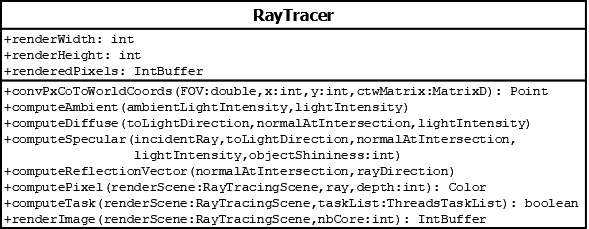
\includegraphics[width=\textwidth]{diagrammes/classe_RayTracer.png}}
	
	\caption{Diagramme de la classe RayTracer et de ses principales méthodes}
	\label{diagrammeRayTracer}
\end{figure}
\FloatBarrier

Les sources de lumière, la caméra et les objets de la scène dont a besoin le RayTracer sont des attributs de RayTracingScene. Comme énoncé plus haut, on peut ainsi facilement les modifier dynamiquement pendant le rendu.

\begin{figure}[h!]
	\adjustbox{center}{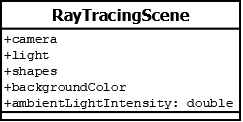
\includegraphics[width=0.42\textwidth]{diagrammes/classe_RayTracingScene.png}}
	
	\caption{Diagramme de la classe RayTracingScene}
	\label{diagrammeRayTracingScene}
\end{figure}
\FloatBarrier

La classe Camera, l'interface Light et la classe RayTracingScene s'organisent toutes dans le package scene:

\begin{figure}[h!]
	\adjustbox{center}{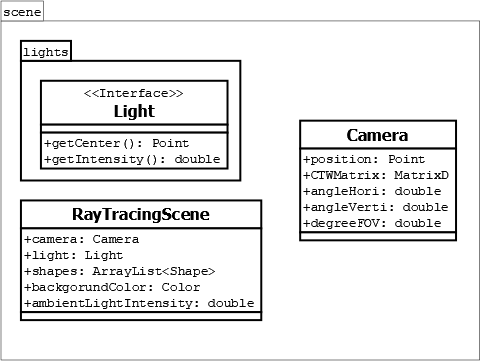
\includegraphics[width=0.75\textwidth]{diagrammes/package_scene.png}}
	
	\caption{Diagramme du package scene}
	\label{diagrammePackageScene}
\end{figure}
\FloatBarrier

\subsubsection{Le package materials}

Afin de colorer notre scène, nous devons donner une couleur aux formes des objets qui composent la scène. De plus, nous devons indiquer au RayTracer si l'objet est réflexif ou si au contraire il est mat, s'il est spéculaire et si oui à quel point, s'il est diffus...
Nous allons donc organiser toutes ces caractéristiques dans ce que l'on va appeler des matériaux.

\begin{figure}[h!]
	\adjustbox{center}{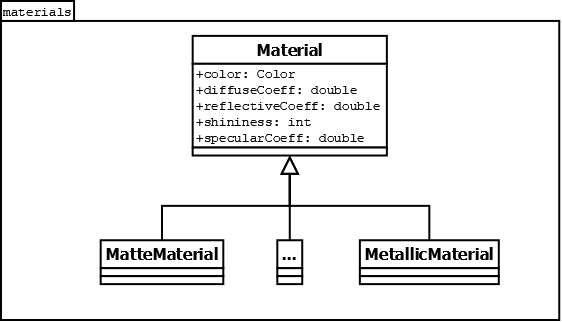
\includegraphics[width=0.75\textwidth]{diagrammes/package_materials.png}}
	
	\caption{Diagramme du package materials}
	\label{diagrammePackageMaterials}
\end{figure}
\FloatBarrier

Une classe mère Material permet de définir un matériau complètement arbitrairement. Toutes les caractéristiques peuvent être choisies comme on le souhaite.\\
Différentes classes héritent ensuite de cette classe mère afin de définir des catégories de matériau. Par exemple, MettalicMaterial va fixer la réflectivité du matériau à un certain point, de même pour sa diffusion, sa spécularité etc... Toutes ces caractéristiques fixées d'une certaine façon donnera donc au matériau un aspect métallique. Il ne restera plus qu'à donner un MetallicMaterial à un objet de la scène pour qu'il ait un aspect métallique pendant le rendu. Le visuel des matériaux peut donc être personnalisé assez facilement et intuitivement avec l'utilisation des matériaux.

\subsubsection{Le package geometry}
\cite{scratchapixel}

\bibliographystyle{unsrt}
\bibliography{bibliography/sources}

\end{document}